% Compile twice with pdfLaTeX. Figures and bibliography are included.
% Source materials: AI教練提案解析.pdf, AI_Fitness_Coach.png, A2Z outline example.pdf
\documentclass[conference]{IEEEtran}
\usepackage{amsmath,booktabs,tabularx,array,tikz,algorithmic}
\usetikzlibrary{arrows.meta,positioning}
\usepackage[hidelinks]{hyperref}
\newcolumntype{Y}{>{\raggedright\arraybackslash}X}
\tikzset{box/.style={draw,rounded corners=2pt,align=center,inner sep=4pt,font=\footnotesize},link/.style={-{Stealth[length=4pt]},thin}}
\begin{document}
\title{AI Fitness Coach: A Conversational Running Coach for Quota-Limited Cloud Deployment}
% Replace the draft label with verified author names and affiliations.
\author{\IEEEauthorblockN{Project proposal}}
\maketitle
\begin{abstract}
% A -- Attention getter
In Strava's 2025 survey, 46\% of respondents said they would use AI for sports coaching. One practical question is whether a runner can finish a route before rain is forecast.
% B -- Challenge
On a 5~km loop, a one-minute-per-kilometre pace error shifts the finish by five minutes. A coach that guesses the pace or reuses a forecast for an earlier departure can reverse the answer even when its arithmetic is correct.
% C -- Cure
AI Fitness Coach asks for the missing input and combines the confirmed pace, route length and local forecast in one reply.
% D -- Development
A browser connects a single agent to running and nutrition tools. A scope check and a usage budget govern calls, and the runner can read the reply or hear it through a lip-synchronized avatar.
% E -- Experiments
The project used a scripted demonstration on a free cloud tier. We specify a follow-up comparison with a form and a locally deployed agent to measure correct task completion, token use and response time.
% F -- Findings
The project reports an end-to-end run spanning conversation, weather and route lookup, manual exercise logging, food analysis, menu retrieval and avatar playback. The demonstration establishes that these functions ran together. Per-attempt measurements are still needed to determine whether page queries meet the proposed 2~s target and spoken replies the 12~s target at the 95th percentile.
\end{abstract}
\begin{IEEEkeywords}
conversational agents, running, tool calling, voice interaction, latency
\end{IEEEkeywords}
\section{Introduction}
Strava's 2025 report drew on a survey of more than 30,000 people, including users and non-users of its platform. Among respondents, 46\% expressed willingness to use AI for sports coaching~\cite{strava}. This measures stated interest. Whether a runner can act on a particular reply depends on how the coach handles details the runner leaves out.

Consider a runner asking if their usual loop fits before the rain. A route planner can supply the distance and a weather service can supply the forecast. The runner still has to combine them with a departure time and a realistic pace. Table~\ref{tab:margin} shows why the coach should ask for pace. At 6:00 min/km the runner has two minutes to spare. At 6:30 min/km the same route takes half a minute too long. Asking again for an already confirmed distance, by comparison, would cost a turn without resolving the decision.

\begin{table}[!b]
\caption{Illustrative 5~km loop starting at 17:00 with rain forecast at 17:32. Positive margin means finishing before forecast onset.}
\label{tab:margin}\centering\small
\begin{tabular}{@{}lrrr@{}}\toprule
Pace (min/km) & Run (min:s) & Finish & Margin (min:s)\\\midrule
6:00 & 30:00 & 17:30:00 & $+$2:00\\
6:30 & 32:30 & 17:32:30 & $-$0:30\\
7:00 & 35:00 & 17:35:00 & $-$3:00\\\bottomrule
\end{tabular}
\end{table}
These examples assume constant pace and no stops. If the weather service gives an onset window, the reply should retain it. An uncertainty of several minutes can erase the two-minute margin in the first row.
The coach supports run interpretation, pace calculation, weather and route lookup, and meal queries~\cite{proposal}. Sections~II and III give the evidence and system design. Section~IV specifies the comparison and Section~V describes the remaining work.

\section{Related Work}
ReAct lets an agent revise its next action after observing a tool result~\cite{react}. This matters when a runner changes the departure time after a forecast lookup. PH-LLM used expert assessments of replies about wearable data~\cite{phllm}, a precedent for checking content separately from fluency.

El Helou \emph{et al.} analyzed 1,791,972 finish records from 60 marathons in six cities over 2001--2010~\cite{heat}. Mean running speed fell above the temperature associated with peak speed, which varied by performance level. The study supports checking local conditions. Applying a numerical pace adjustment to a recreational 5~km run would require data for that distance and population. Table~\ref{tab:papers} connects the evidence to design decisions. The open question is whether the coach can give a correct, timely answer when a turn needs both arithmetic and external data.
\begin{table*}[t]
\caption{Evidence informing the agent and the running-domain design}
\label{tab:papers}\centering\small
\begin{tabularx}{\textwidth}{@{}p{2.3cm}YYY@{}}\toprule
Study & Question and method & Data and finding & Implication for the coach\\\midrule
ReAct~\cite{react}, 2023 & Can an agent use external observations to revise a decision? The model alternated reasoning with actions. & On WebShop, task success improved by 10 percentage points over the comparison method. & Retain the observation behind a reply so a changed departure time can trigger a fresh lookup.\\
PH-LLM~\cite{phllm}, 2025 & Can a fine-tuned model interpret wearable summaries for sleep and fitness coaching? & Of 857 cases developed, 100 were held out. On fitness cases, expert raters scored model responses similarly to expert answers. & Rate the content of the coaching reply separately from its delivery time.\\
El Helou et al.~\cite{heat}, 2012 & How did weather relate to running speed? The study linked finish records to race conditions. & Across 60 races, temperature showed the strongest weather association with performance. & Retrieve the local forecast and confirm the individual's pace before estimating finish time.\\\bottomrule
\end{tabularx}
\end{table*}

\section{Proposed System}
\subsection{Architecture and turn processing}
Figure~\ref{fig:arch} shows the five components in the project materials~\cite{project}. The browser accepts text or speech. The backend exposes request--response operations over REST and carries interactive events over WebSocket. ScopeGuard checks whether a request concerns the supported fitness tasks. The agent selects a tool and interprets its output. A session snapshot carries confirmed inputs, tool results and usage into the next turn.

\begin{figure}[htbp]\centering
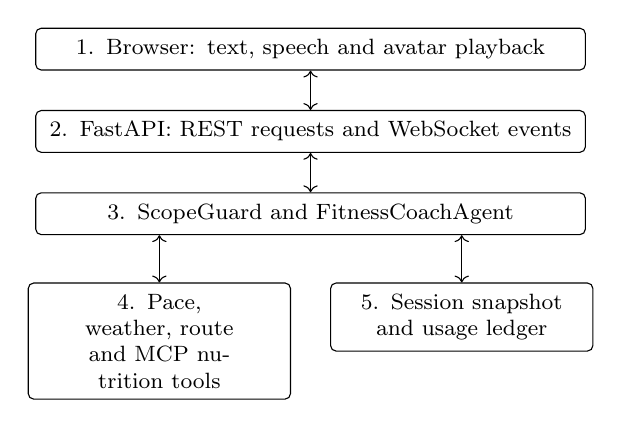
\begin{tikzpicture}[node distance=5mm]
\node[box,text width=6.7cm] (ui) {1. Browser: text, speech and avatar playback};
\node[box,below=of ui,text width=6.7cm] (api) {2. FastAPI: REST requests and WebSocket events};
\node[box,below=of api,text width=6.7cm] (agent) {3. ScopeGuard and FitnessCoachAgent};
\node[box,below=6mm of agent,xshift=-1.92cm,text width=3.05cm] (tools) {4. Pace, weather, route\\and MCP nutrition tools};
\node[box,below=6mm of agent,xshift=1.92cm,text width=3.05cm] (db) {5. Session snapshot\\and usage ledger};
\draw[<->] (ui)--(api);\draw[<->] (api)--(agent);
\draw[<->] (agent.south -| tools.north)--(tools.north);
\draw[<->] (agent.south -| db.north)--(db.north);
\end{tikzpicture}
\caption{The browser receives replies through the API. The agent accesses domain tools and persistent session state separately. MCP denotes Model Context Protocol.}\label{fig:arch}
\end{figure}

For a run with duration $t$ in minutes and distance $d>0$ in kilometres, pace is $p=t/d$ in minutes per kilometre. A 30-minute run over 5 km yields 6:00 min/km. Rounding is deferred until display. If the runner gives a number without a unit, the agent asks for the unit before saving the duration. A forecast additionally requires a place and time. Route length alone cannot resolve which forecast to use.

Figure~\ref{fig:flow} distinguishes requests that need clarification from requests ready for a tool. Algorithm~1 specifies a proposed accounting rule. Before a billable call, reserve an upper bound $r$ on its token cost. If actual usage is $u\leq r$, release $r-u$ tokens. With starting balance $B$, the resulting balance is $B-u$. A timeout with unknown usage keeps its reservation until reconciliation. Atomic reservations prevent two turns from spending the same balance.

\begin{figure}[htbp]\centering
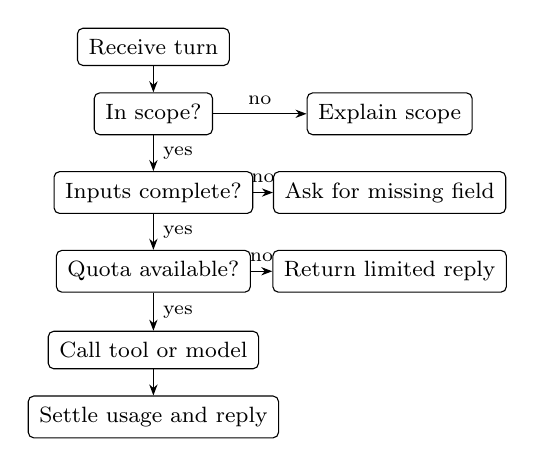
\begin{tikzpicture}
\node[box] (input) at (0,0) {Receive turn};
\node[box] (scope) at (0,-.85) {In scope?};
\node[box] (fields) at (0,-1.85) {Inputs complete?};
\node[box] (budget) at (0,-2.85) {Quota available?};
\node[box] (work) at (0,-3.85) {Call tool or model};
\node[box] (reply) at (0,-4.7) {Settle usage and reply};
\node[box] (redirect) at (3,-.85) {Explain scope};
\node[box] (ask) at (3,-1.85) {Ask for missing field};
\node[box] (stop) at (3,-2.85) {Return limited reply};
\draw[link] (input)--(scope);
\foreach \a/\b in {scope/fields,fields/budget,budget/work}{\draw[link] (\a)--node[right,font=\scriptsize]{yes}(\b);}
\foreach \a/\b in {scope/redirect,fields/ask,budget/stop}{\draw[link] (\a)--node[above,font=\scriptsize]{no}(\b);}
\draw[link] (work)--(reply);
\end{tikzpicture}
\caption{Decision path for one turn. Each right-hand branch returns control to the runner.}\label{fig:flow}
\end{figure}

\par\smallskip\noindent\textbf{Algorithm 1. Processing a coaching turn}\par
\begin{algorithmic}[1]
\STATE Load the snapshot and any completed reply for the turn ID.
\IF{the turn already has a completed reply}
  \STATE Return the stored reply.
\ENDIF
\STATE Apply ScopeGuard. Return guidance if outside scope.
\STATE Resolve units, place and time required by the intent.
\IF{a required field is missing}
  \STATE Save the pending intent, ask for the field and end turn.
\ENDIF
\FOR{each required call, up to the turn limit}
  \STATE Reserve its cost bound atomically or return a quota notice.
  \STATE Invoke the call and record the result or error.
  \STATE Settle known usage or flag the reservation for reconciliation.
  \IF{enough evidence is available, or a required call failed}
    \STATE Exit loop.
  \ENDIF
\ENDFOR
\STATE Save the evidence and reply under the turn ID.
\STATE Return text and, when requested and available, speech.
\end{algorithmic}

\subsection{Design tradeoffs}
The design preserves units, checks forecast validity, traces claims to tool outputs, reserves quota and retains confirmed inputs after reconnection. Three tradeoffs follow. Free-form requests can omit units, so the coach asks before calculating. A single agent shares context across tasks, so tools receive only the fields they need. Streaming can shorten the wait but can also speak an obsolete estimate, so numerical replies wait for the required evidence.

\section{Evaluation Protocol}
The original proposal describes a first-stage demonstration using a scripted account~\cite{proposal,project}. It connects an initial planning query to weather and route retrieval, adopting a plan, entering a run manually, correcting a food entry and retrieving the saved record. This is evidence that information can pass between functions. The proposal gives no attempt counts or turn-level logs from which to calculate a success rate, latency percentile or token saving. The protocol below specifies what to collect on the next run.
\subsection{Comparisons and measurement}
Run the same tasks through a form interface, the cloud agent and a local deployment of the same agent. For both agent deployments, fix the model, prompts, tool responses and token cap where possible. Test live services separately to expose network variation. Compare all three on field accuracy and task completion. Compare voice onset across voice-capable configurations. Report cold starts separately from warm turns, and retain failed turns in the completion denominator.

For the two shared tasks (computing pace and selecting a forecast for a revised departure), the minimum planned comparison is $2$ tasks $\times$ $3$ configurations $\times$ $30$ repetitions, or 180 attempts at one fixed load and start condition. Match inputs and rotate configuration order. Run voice and injected failures separately on applicable configurations. To isolate avatar overhead, repeat the same voice request with lip synchronization enabled and disabled. Scripted repetitions measure service behavior under the chosen conditions. Estimating time saved by runners would require observing runners using the interfaces.

Table~\ref{tab:metrics} defines the four timing endpoints in the project proposal~\cite{proposal}. Within each condition, sort the $n$ successful timed trials and take rank $\lceil0.95n\rceil$ for P95. With 30 successes, P95 is the second-slowest time. If only 24 of 30 attempts succeed, the latency summary covers those 24 and completion is 80\%. If none succeeds, P95 is undefined. Publish the denominators beside the timings. Vary the token cap and concurrency to identify where either completion or latency deteriorates.

\begin{table}[tb]
\caption{Proposed response targets. Clocks start and stop at the client. The first three targets apply to P95.}
\label{tab:metrics}\centering\footnotesize
\begin{tabularx}{\columnwidth}{@{}lYr@{}}\toprule
Interaction & Timing interval & Target\\\midrule
Page query & Submit to visible data & $<2$~s\\
Text reply & Submit to first text that addresses the task & $<8$~s\\
Voice reply & End of speech to first audible reply & $<12$~s\\
Interrupt & Stop command to playback silence & $<300$~ms\\\bottomrule
\end{tabularx}
\end{table}

Score each attempted task against the expected outcome below. For valid pace inputs, report absolute error in seconds per kilometre against $60t/d$ and count missing replies separately. For forecast tasks, check both the location and the validity interval. Record clarification turns per attempt. Divide all billed tokens, including those spent on failed attempts, by the number of completed tasks. For factual replies, report the fraction whose material claims all trace to valid tool results or confirmed inputs. These measures expose cases in which a quick reply is incomplete or a low token count reflects an early failure.
\subsection{Ten questions for validating the coach}
Each question has an observable answer for a scripted test.
\begin{enumerate}
\item What pace follows from 5 km in 30 min? The expected value is 6:00 min/km.
\item How is zero distance handled? The client requests a positive distance and displays no pace.
\item What happens when units are omitted? The next turn asks for the unit and preserves the number.
\item Which forecast fits a changed departure time? Its validity interval must cover the updated time at the requested location.
\item What if a route lookup times out? The reply identifies the missing route and omits its length.
\item Where did a meal estimate come from? The trace links it to an MCP result and its portion size.
\item Does an unrelated request use a domain tool? The trace ends at ScopeGuard before such a call runs.
\item Can concurrent turns exceed the balance? Settled usage plus active reservations must stay within the starting quota.
\item Does reconnecting duplicate a completed turn? Resubmitting its ID returns the stored reply and leaves the ledger unchanged.
\item When does the avatar respond? Record the offset between first audible speech and first mouth motion separately from voice onset.
\end{enumerate}
Unit tests check arithmetic and quota updates. Integration tests inject stale forecasts, timeouts and duplicate IDs. A browser smoke test covers spoken input through playback.

\section{Conclusion}
The demonstration linked a runner's question to tools and a spoken reply. The proposed comparison will show when that reply arrives in time, when it is correct and how often quota limits interrupt the task. GPS, step counts and posture sensing remain future work and require separate validation.

\begin{thebibliography}{00}
\bibitem{strava} Strava, \emph{12th Annual Year in Sport Trend Report}, Dec. 3, 2025. \href{https://press.strava.com/en-gb/articles/strava-releases-12th-annual-year-in-sport-trend-report-2025}{Online report}.
\bibitem{proposal} \emph{AI Fitness Coach: A Conversational Running Coach}, original course proposal, Nov. 10, 2026, in Chinese, pp. 1--4. \href{https://github.com/HitomiHuang/DIC3-AI-Fitness-Coach/blob/main/myplan/proposal.pdf}{Project proposal}.
\bibitem{project} \emph{AI Fitness Coach Proposal Analysis}, course project review, pp. 1--2, undated, in Chinese. Supplied with the project infographic.
\bibitem{react} S. Yao \emph{et al.}, \textquotedblleft ReAct: Synergizing reasoning and acting in language models,\textquotedblright\ in \emph{Proc. Int. Conf. Learning Representations}, 2023. \href{https://react-lm.github.io/}{Project and paper}.
\bibitem{phllm} J. Khasentino \emph{et al.}, \textquotedblleft A personal health large language model for sleep and fitness coaching,\textquotedblright\ \emph{Nature Medicine}, vol. 31, pp. 3394--3403, 2025, \href{https://doi.org/10.1038/s41591-025-03888-0}{doi: 10.1038/s41591-025-03888-0}.
\bibitem{heat} N. El Helou \emph{et al.}, \textquotedblleft Impact of environmental parameters on marathon running performance,\textquotedblright\ \emph{PLOS ONE}, vol. 7, no. 5, Art. no. e37407, 2012, \href{https://doi.org/10.1371/journal.pone.0037407}{doi: 10.1371/journal.pone.0037407}.
\end{thebibliography}
\end{document}
